\documentclass[11pt,letterpaper]{article}
\usepackage[letterpaper, margin=1in]{geometry}
\usepackage[T1]{fontenc}
\usepackage[utf8]{inputenc}
\usepackage[english]{babel}
\usepackage{natbib,latexsym}
\bibliographystyle{plainnat}
\usepackage{graphicx}
\usepackage{hyperref}
\hypersetup{
    colorlinks=true,
    linkcolor=blue,
    filecolor=magenta,      
    urlcolor=cyan,
}
\title{Triplet Extraction from sentences}

\author{Sumith Baddam, Deepthi Raghu, Third Author, ... \\
  Affiliation
  {\tt \{srbaddam, draghu, email3, ...\}@iu.edu} \\}

\date{\today}

\begin{document}
\maketitle

\begin{abstract}
  In this paper we present an approach for extracting triplets from sentences using Json-NLP semantic relationship extractor and dependency parser. Triplet extraction is the processing of extracting subject-verb-object relationships from multiple sentences. This paper presents various traditional approaches previously used by others and evaluates our approach. We further compares our results with the results from traditional approaches. We would also discuss the evaluation procedure we followed and the challenges we faced in this project.
\end{abstract}

\section{Introduction}

Triplet Extraction is a crucial cog in the field of Natural Language Processing (NLP) and linguistics. It’s widely used for tasks such as Question Answering Systems, Machine Translation, Entity Extraction, Event Extraction, Named Entity Linking, Co-reference Resolution, Relation Extraction, etc.\\

A triplet represents a couple of entities and a relation between them. For example, (Damir Cavar, teach, NLP course) is a triple in which ‘Damir Cavar’ and ‘NLP course’ are the related entities, and the relation between them is ‘teach’. In this paper, we will focus on the extraction of these types of triples from a given text.\\

The main scope of this project is the triple extraction from sentences. Three relation types are explored.

\begin{itemize}
    \item (subject, verb, object)
    \item (event, occurs after, event)
    \item (event, preposition, proposition object)
\end{itemize}

This problem requires understanding large corpora, which is an increasingly popular problem these days. In this report, we will discuss and explain some Natural Language Processing (NLP) techniques that we used to extract the subject, verb and object of a particular sentence and the different approaches used in particular by our team.


\section{Previous Work}
Our research about the previous work for this task exposed us to two different approaches. Traditional triplet extraction and open triplets extraction. In Traditional Extraction, the relations to be extracted are pre-defined. In Open Extraction, the relations are not pre-defined. The system is free to extract any relations it comes across while going through the text data. We also came across different methods from some of the research papers we read. Although many of these approaches involved building a neural model, we mainly focused on approaching the problem of triple extraction using a linguistic method (rule based extraction).

\subsection{Semantic Relationships: Get Structured Knowledge from Unstructured Text}
Let's have a look at text snippet, “Food Tutorials are better when directed by Wes Anderson. Bruce Lee's biopic, 'Little Dragon' to be directed by Shekhar Kapur.” \\

In the first sentence, we have two entities (“Food Tutorials” and “Wes Anderson”). These entities are related by the term “Directed”. Hence, (Wes Anderson, directed, Food Tutorials) is a triple.Similarly, we can extract relations from the other sentences as well, (Shekhar Kapur, directed, Little dragon). It turns out that we can get structured information based on the syntactic structure and grammar of the text, as illustrated in the example above.

\subsection{Different Approaches to Triplet Extraction}
In the previous section, we managed to easily extract triples from a few sentences. However, in the real world, the data size is huge and manual extraction of structured information is not feasible. Therefore, automating this information extraction becomes important.\\

There are multiple approaches to perform information extraction automatically. Let’s understand them one-by-one:
\begin{itemize}
    \item \textbf{Rule-based Approach:} We define a set of rules for the syntax and other grammatical properties of a natural language and then use these rules to extract information from text. 
    \item \textbf{Supervised:} Let’s say we have a sentence S. It has two entities E1 and E2. Now, the supervised machine learning model has to detect whether there is any relation (R) between E1 and E2. So, in a supervised approach, the task of relation extraction turns into the task of relation detection. The only drawback of this approach is that it needs a lot of labeled data to train a model.
    \item \textbf{Semi-supervised:} When we don’t have enough labeled data, we can use a set of seed examples (triples) to formulate high-precision patterns that can be used to extract more relations from the text.

\end{itemize}

\section{Approach}
For this task, we used NLTK, JSON-NLP and requests framework. We extract structured information from unstructured data (text data in our case). We’ve already seen that the information in text lies in the form of relations between different entities. \subsection{Subtree Matching for triplet extraction}
Our methodology is similar to subtree matching for relation extraction.\\

The simple rule-based methods work well for information extraction tasks. However, they have a few drawbacks and shortcomings. We have to be extremely creative to come up with new rules to capture different patterns. It is difficult to build patterns that generalize well across different sentences. To enhance the rule-based methods for relation/information extraction, we should try to understand the dependency structure of the sentences at hand. We use JSON-NLP API for getting the dependency structure of the sentence. From the output of the API, we try to find interesting relationships. \\

For example, let's consider the sentence to be, “Tableau was recently acquired by Salesforce.” Output from the API is <Image>\\

If you look at the entities in the sentence – Tableau and Salesforce – they are related by the term ‘acquired’. So, the pattern I can extract from this sentence is either “Salesforce acquired Tableau” or “X acquired Y”.\\

Now consider another statement, “Careem, a ride-hailing major in the middle east, was acquired by Uber.” Output from the API is <Image>\\

From the graph, all we have to check is which dependency paths are common between multiple sentences. This method is known as Subtree matching. We will just consider the common dependency paths and extract the entities and the relation (acquired) between them. Hence, the relations extracted from these sentences are:
\begin{itemize}
    \item Salesforce acquired Tableau
    \item Uber acquired Careem
\end{itemize}

After extracting a basic subject - verb - object extracted from a single sentence by the above approach, we had to handle compounds such as adjectives and modifiers. Also, we had to handle sentences with multiple subject/verb/object occurrences, define a particular output structure and handle reading multiple files containing multiple sentences. In addition to this, event ordering also had to be included. The various experiments done to achieve these results have been described in the next section. 

\section{Experiments}
To bring in some creativity, we developed two different rule-based methods to handle the triple extraction. One of our approaches was to extend the base code that extracts a single subject/verb/object and write rules to identify compounds such as adjectives and modifiers from the dependency tree. 

\noindent
The rules are specifically based on the 'tokenlist' and the 'dependency' parts of the JSON from the NLP-API. In this approach, we take as input, a list of files containing multiple sentences line by line. The output will be a list of JSONs corresponding to each sentence in the input files. \\

\noindent
For example, if the input is a file containing two sentences:

"Mary marinated the chicken." 

"John cooked the chicken."

\noindent \newline
Then the output will be:

\{'sentence': 1, 'event': 1, 'subject': 'Mary', 'verb': 'marinate', 'object': 'chicken'\}

\{'sentence': 2, 'event': 2, 'subject': 'John', 'verb': 'cook', 'object': 'chicken'\}

\noindent \newline
Explanation of output:
\begin{itemize}
    \item The sentence key in the output JSON provides a reference to the sentence number in the input sentence file.
    
    \item The event key in the output JSON indicates the event ordering i.e, the ordering of the predicates.
    
    \item The subject, verb and object keys indicate the triples that have been extracted.
\end{itemize}
The rules were extended as and when new scenarios and variations of the triples have to be handled.
Below are some example sentences from file15.txt in webanno to show the different variations handled:
\begin{enumerate}
    \item
    \textbf{Sentence:} Prepare the cake mixes according to the package directions. \newline
    \textbf{Variation in triple:} This sentence has a compound object 'cake mixes'.
    \newline
    \textbf{Extracted output:} 
    
    \{'sentence': 1, 'event': 1, 'subject': '<imperative-chef>', 'verb': 'prepare', 'object': 'cake mix'\}
    \newline
    \textbf{Inference from output:} 
    An important point to note is that in sentences that do not have a subject, we replace the subject with "<imperative-chef>". In this particular example, we can see that the compound object "cake mix" has been extracted successfully.
    
    \item
    \textbf{Sentence:} Stir to combine, then add the milk, cream and butter.
    \newline
    \textbf{Variation in triple:} This sentence has a multiple objects - milk, cream, butter
    \newline
    \textbf{Extracted output:} 
    
    \{'sentence': 1, 'event': 1, 'subject': '<imperative-chef>', 'verb': 'add', 'object': 'milk'\}
    
    \{'sentence': 1, 'event': 1, 'subject': '<imperative-chef>', 'verb': 'add', 'object': 'cream'\}
    
    \{'sentence': 1, 'event': 1, 'subject': '<imperative-chef>', 'verb': 'add', 'object': 'butter'\}
    
    \textbf{Inference from output:} 
    Whenever there are multiple subjects/verbs/objects, our approach will naively produce all combinations of triples. In this case, the three objects, milk, cream and butter have been identified and put into three different triples. Since all the extracted triples are from the same sentence, the sentence key remains unchanged.
    
    \item
    \textbf{Sentence:} Cover and cook until cauliflower begins to soften, about 4 minutes.
    \newline
    \textbf{Variation in triple:} This sentence has a multiple verbs - cover, cook and it has no object
    \newline
    \textbf{Extracted output:} 
    
    \{'sentence': 1, 'event': 1, 'subject': 'cauliflower', 'verb': 'cover', 'object': '<None>'\}
    
    \{'sentence': 1, 'event': 2, 'subject': 'cauliflower', 'verb': 'cook', 'object': '<None>'\}
    
    \textbf{Inference from output:} 
    Whenever there are multiple subjects/verbs/objects, our approach will naively produce all combinations of triples. In this case, the two verbs cover and cook have been identified and put into two different triples. Also, since this sentence does not have an object, we replace the object with '<None>'. Another point to note here is that since there are two verbs in this sentence, the event changes accordingly, capturing the order in which the actions occurred.

\end{enumerate}

\noindent
In this manner, multiple files containing multiple sentences line by line can be processed to produce an output JSON. 

\noindent \newline
\textbf{Steps to run the code for this experiment:}
\begin{itemize}
    \item Run the python code \textbf{extract\_triples\_deepthi.py} using the command:
    
    \textbf{python extract\_triples\_deepthi.py file1.txt file2.txt ...}
    
    where, file1.txt, file2.txt .. are the input files
    
    \item After the execution of code, the result is generated in the file \textbf{Result\_JSON.txt}
\end{itemize}

\noindent
In order to standardize the outputs of all the experiments, we decided to utilize the graph.py code to give a graph object as the output. To incorporate this output format, we modified the existing \textbf{extract\_triples\_deepthi.py} into \textbf{extract\_triples\_graph\_deepthi.py} and constructed two relations:

\begin{itemize}
    \item Triples (Subject, Verb, Object)
    \item Event relation (Event2 occurs\_after Event1)
\end{itemize}

\noindent
The graph.py enabled us to produce two types of results:
\begin{enumerate}
    \item A graph object represented as a JSON 
    \item A line by line relation extraction
\end{enumerate}
\noindent
We produced both these outputs. Below is an example:
\noindent \newline
\textbf{Sentences:} 

Prepare the cake mixes according to the package directions.

Stir to combine, then add the milk, cream and butter.

\noindent 
\textbf{Extracted output1 : A graph object represented as a JSON } 
\newline

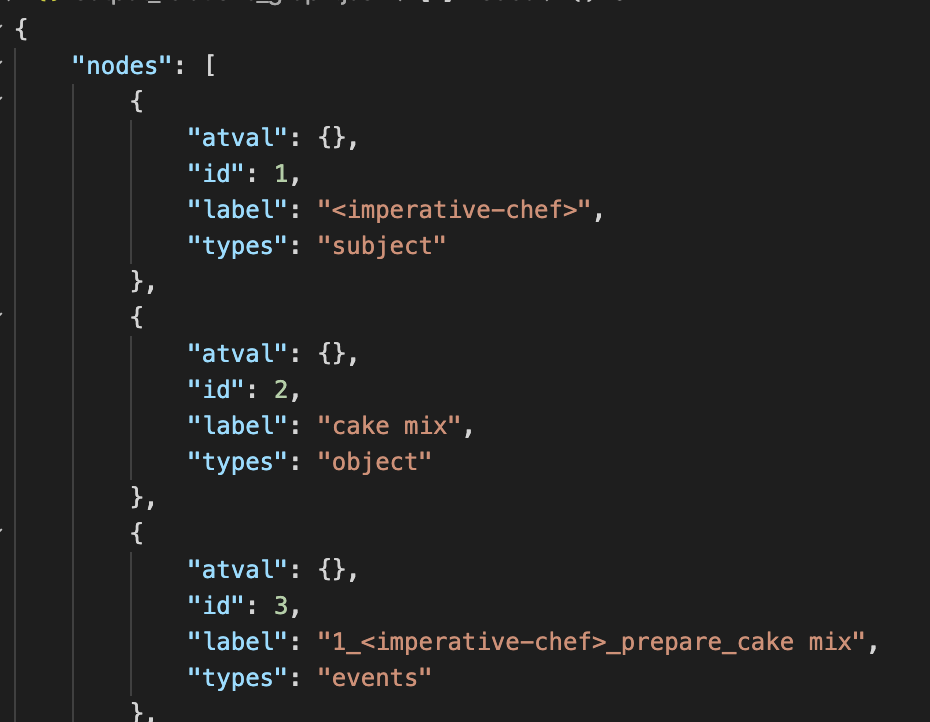
\includegraphics[width=9cm, height=9cm]{graph_obj1.png}
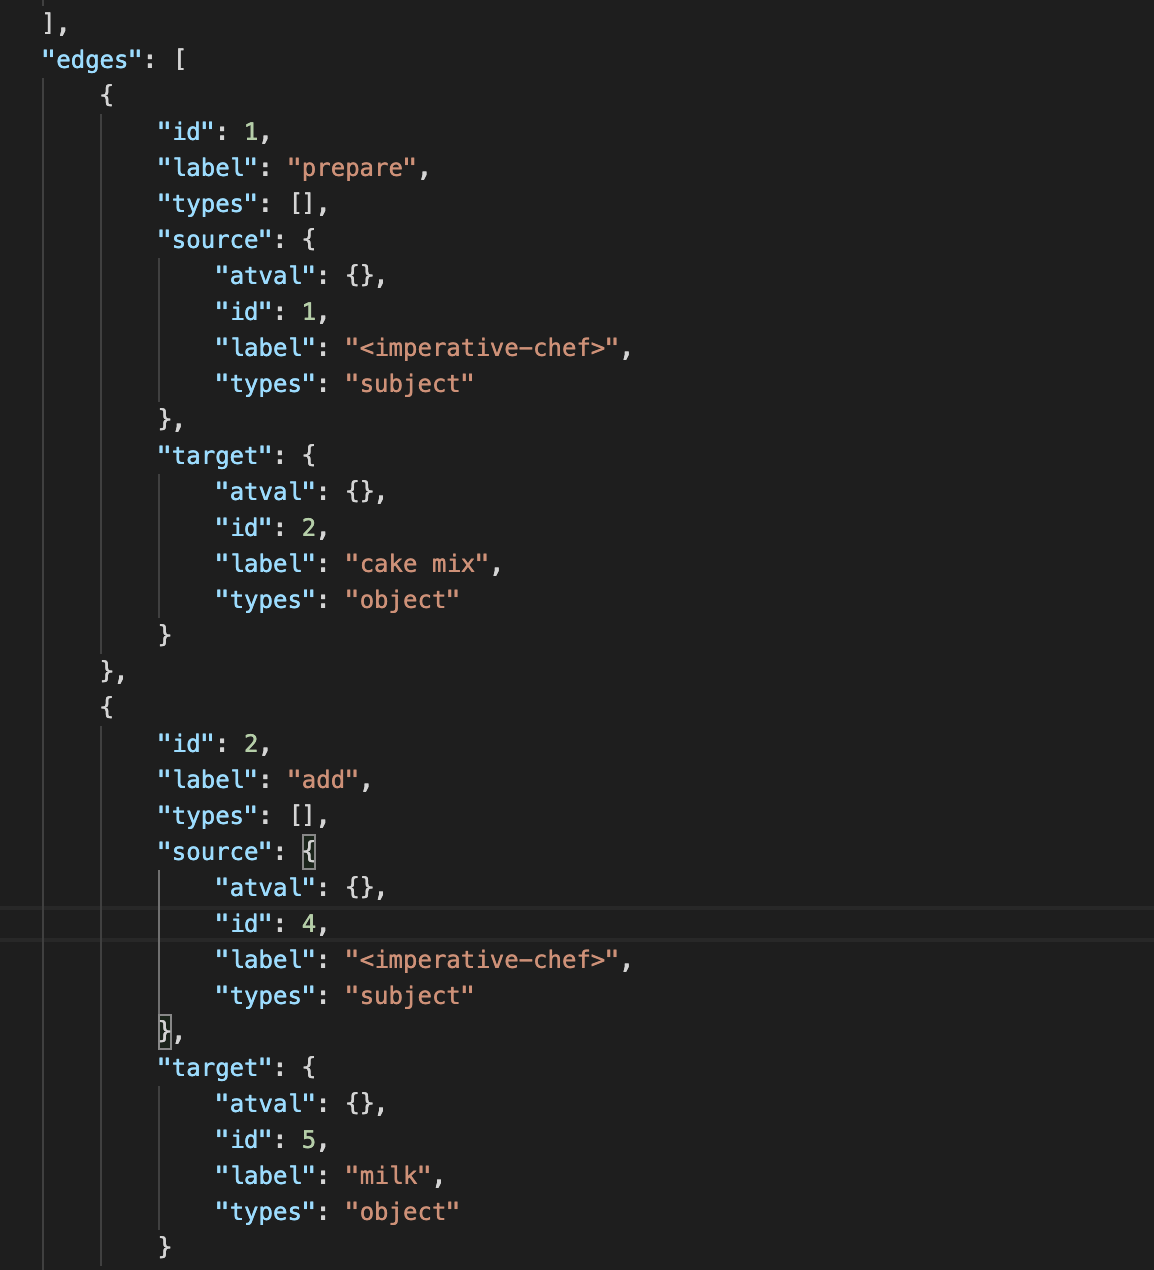
\includegraphics[width=9cm, height=9cm]{graph_obj2.png}

\noindent
\textbf{Extracted output2 : A line by line relation extraction } 

\begin{flushleft}
\{'source': '<imperative-chef>', 'relation': 'prepare', 'target': 'cake mix'\}

\{'source': '<imperative-chef>', 'relation': 'add', 'target': 'milk'\}

\{'source': '<imperative-chef>', 'relation': 'add', 'target': 'cream'\}

\{'source': '<imperative-chef>', 'relation': 'add', 'target': 'butter'\}

\{'source': '2\_<imperative-chef>\_add\_milk', 'relation': 'occurs\_after', 'target': '1\_<imperative-chef>\_prepare\_cake mix'\}

\{'source': '3\_<imperative-chef>\_add\_cream', 'relation': 'occurs\_after', 'target': '2\_<imperative-chef>\_add\_milk'\}

\{'source': '4\_<imperative-chef>\_add\_butter', 'relation': 'occurs\_after', 'target': '3\_<imperative-chef>\_add\_cream'\}

\end{flushleft}
\noindent 
\textbf{Inference from output1:} 

In the graph object, Subjects, Objects and Events are constructed as nodes. An edge is drawn in two cases:
\begin{enumerate}
    \item Edge over a verb, connecting a subject and an object to capture triple relations
    \item Edge over "occur\_after", connecting two events to capture event relations
\end{enumerate}
\noindent 
\textbf{Inference from output2:} 

This output gives a line by line relation extraction. It extracts two relations:

\begin{itemize}
    \item Triple relations like \{'source': '<imperative-chef>', 'relation': 'add', 'target': 'milk'\}
    \item Event relations like \{'source': '3\_<imperative-chef>\_add\_cream', 'relation': 'occurs\_after', 'target': '2\_<imperative-chef>\_add\_milk'\}
    
\end{itemize}
\noindent \newline
Also, in this experiment, the event ID has been generated by concatinating the verb ID from its corresponding graph node with with subject, verb and object as "verbID\_subject\_verb\_object to get a unique event ID.

\noindent \newline
\textbf{Steps to run the code for this experiment:}
\begin{itemize}
    \item Run the python code \textbf{extract\_triples\_graph\_deepthi.py} using the command:
    
    \textbf{python extract\_triples\_graph\_deepthi.py file1.txt file2.txt ...}
    
    where, file1.txt, file2.txt .. are the input files
    
    \item After execution of the code, the graph object (output1) is generated in \textbf{output\_relations\_graph.json} and the line by line relation extraction (output2) is generated in \textbf{output\_relations\_triples.txt}
\end{itemize}
\section{Experiments}

Our experiments...



\section{Evaluation}

This is how we evaluated our work, presenting the evaluation scores in comparison to previous projects...



\section{Discussion}

The discussion of the issues and...


\subsection{Conclusion}

Some conclusion...


% the bibliography
\bibliography{main}


\end{document}
